%TITLE, AUTHOR, DATE
\documentclass[12pt, a4paper]{article} %14 pt indicates the font size of the prepared document
\usepackage[margin=1in]{geometry}
\usepackage[utf8]{inputenc}
\usepackage{multicol}
\usepackage{multirow}
\usepackage{color}
\usepackage{enumerate}
\usepackage{amsmath}
\usepackage{graphicx}
\usepackage{calligra}
\usepackage{hyperref}
\usepackage{subfigure}
\usepackage{biblatex}
\addbibresource{bibfile.bib}


\title{CSE 300: Online Assignment}
\author{Md Shamsuzzoha Bayzid$^{1,\dagger}$, Mahjabin Nahar$^{1}$, Md Shariful Islam\\ Bhuyan$^{1}$, and Md Saidur Rahman$^{1}$ \\ \\
	$^1$Department of Computer Science and Engineering \\
	Bangladesh University of Engineering and Technology \\
	*Corresponding author: shams bayzid@cse.buet.ac.bd \\
	These authors contributed equally to this work
}
\date{April 2021}

\begin{document}
	\maketitle
	
	\section{Introduction}
	This assignment has been designed to assess the preparation of the students in writing	scientific articles using \LaTeX. Different components, that are frequently used in scientific manuscripts, have been covered in this assignment.
	
	
	\subsection{Tables}
	We wish to place Table 1 right here.
	
	\begin{table}[h]
		\centering
		\caption{\textbf{Optimization scores for Method-1 and Method-2 on different datasets covering various model conditions.} We show average scores of two optimization criteria for various model conditions.}
		
	\vspace{10mm}
	\begin{tabular}{|c|c|c|c|c|c|c|}
	\hline
	\multicolumn{3}{|c|}{Simulation Condition} & \multicolumn{4}{|c|}{Optimization Score}\\ 
	\hline
	\multirow{2}{*}{Dataset} & \multirow{2}{*}{Complexity} & Model & \multicolumn{2}{|c|}{Score 1} & \multicolumn{2}{|c|}{Score 2}\\ 
	\cline{4-7}
	& &	Condition & \multicolumn{2}{|c|}{Method-1 \hspace{5mm} Method-2} & \multicolumn{2}{|c|}{Method-1 \hspace{5mm} Method-2} \\ \hline
	\hline
	
	\multirow{4}{*}{D1} & \multirow{2}{*}{easy} & M1 & \multicolumn{2}{c}{7,425.55 \hspace{10mm}     770.00} & \multicolumn{2}{|c|}{929.55 \hspace{10mm} 10} \\
	& & M2 & \multicolumn{2}{c}{7,425.55 \hspace{10mm}     770.00} & \multicolumn{2}{|c|}{929.55 \hspace{10mm} 20} \\
	\cline{2-7}
	
	 & \multirow{2}{*}{hard} & M3 & \multicolumn{2}{c}{7,425.55 \hspace{10mm} 770.00} & \multicolumn{2}{|c|}{929.55 \hspace{10mm} 34}\\
	& & M4 &\multicolumn{2}{c}{7,425.55 \hspace{10mm} 770.00} & \multicolumn{2}{|c|}{929.55 \hspace{10mm} 10} \\
	\hline
	\hline
	
	\multirow{3}{*}{D3} & \multirow{3}{*}{Moderate} &M1 & \multicolumn{2}{c}{7,425.55 \hspace{10mm}     770.00}& \multicolumn{2}{|c|}{929.55 \hspace{10mm} 10}\\
	
	& & M2 & \multicolumn{2}{c}{Not Applicable} & \multicolumn{2}{|c|}{929.55 \hspace{10mm} 10}\\
	& & M3 &\multicolumn{2}{c}{7,425.55 \hspace{10mm}     770.00} & \multicolumn{2}{|c|}{929.55 \hspace{10mm} 10} \\
	\cline{1-7}	
			
		\end{tabular}
	\end{table}
	\newpage
	
	%% add a pdf file/figure
	
	\begin{figure}[h!]
		%...
		\centering
		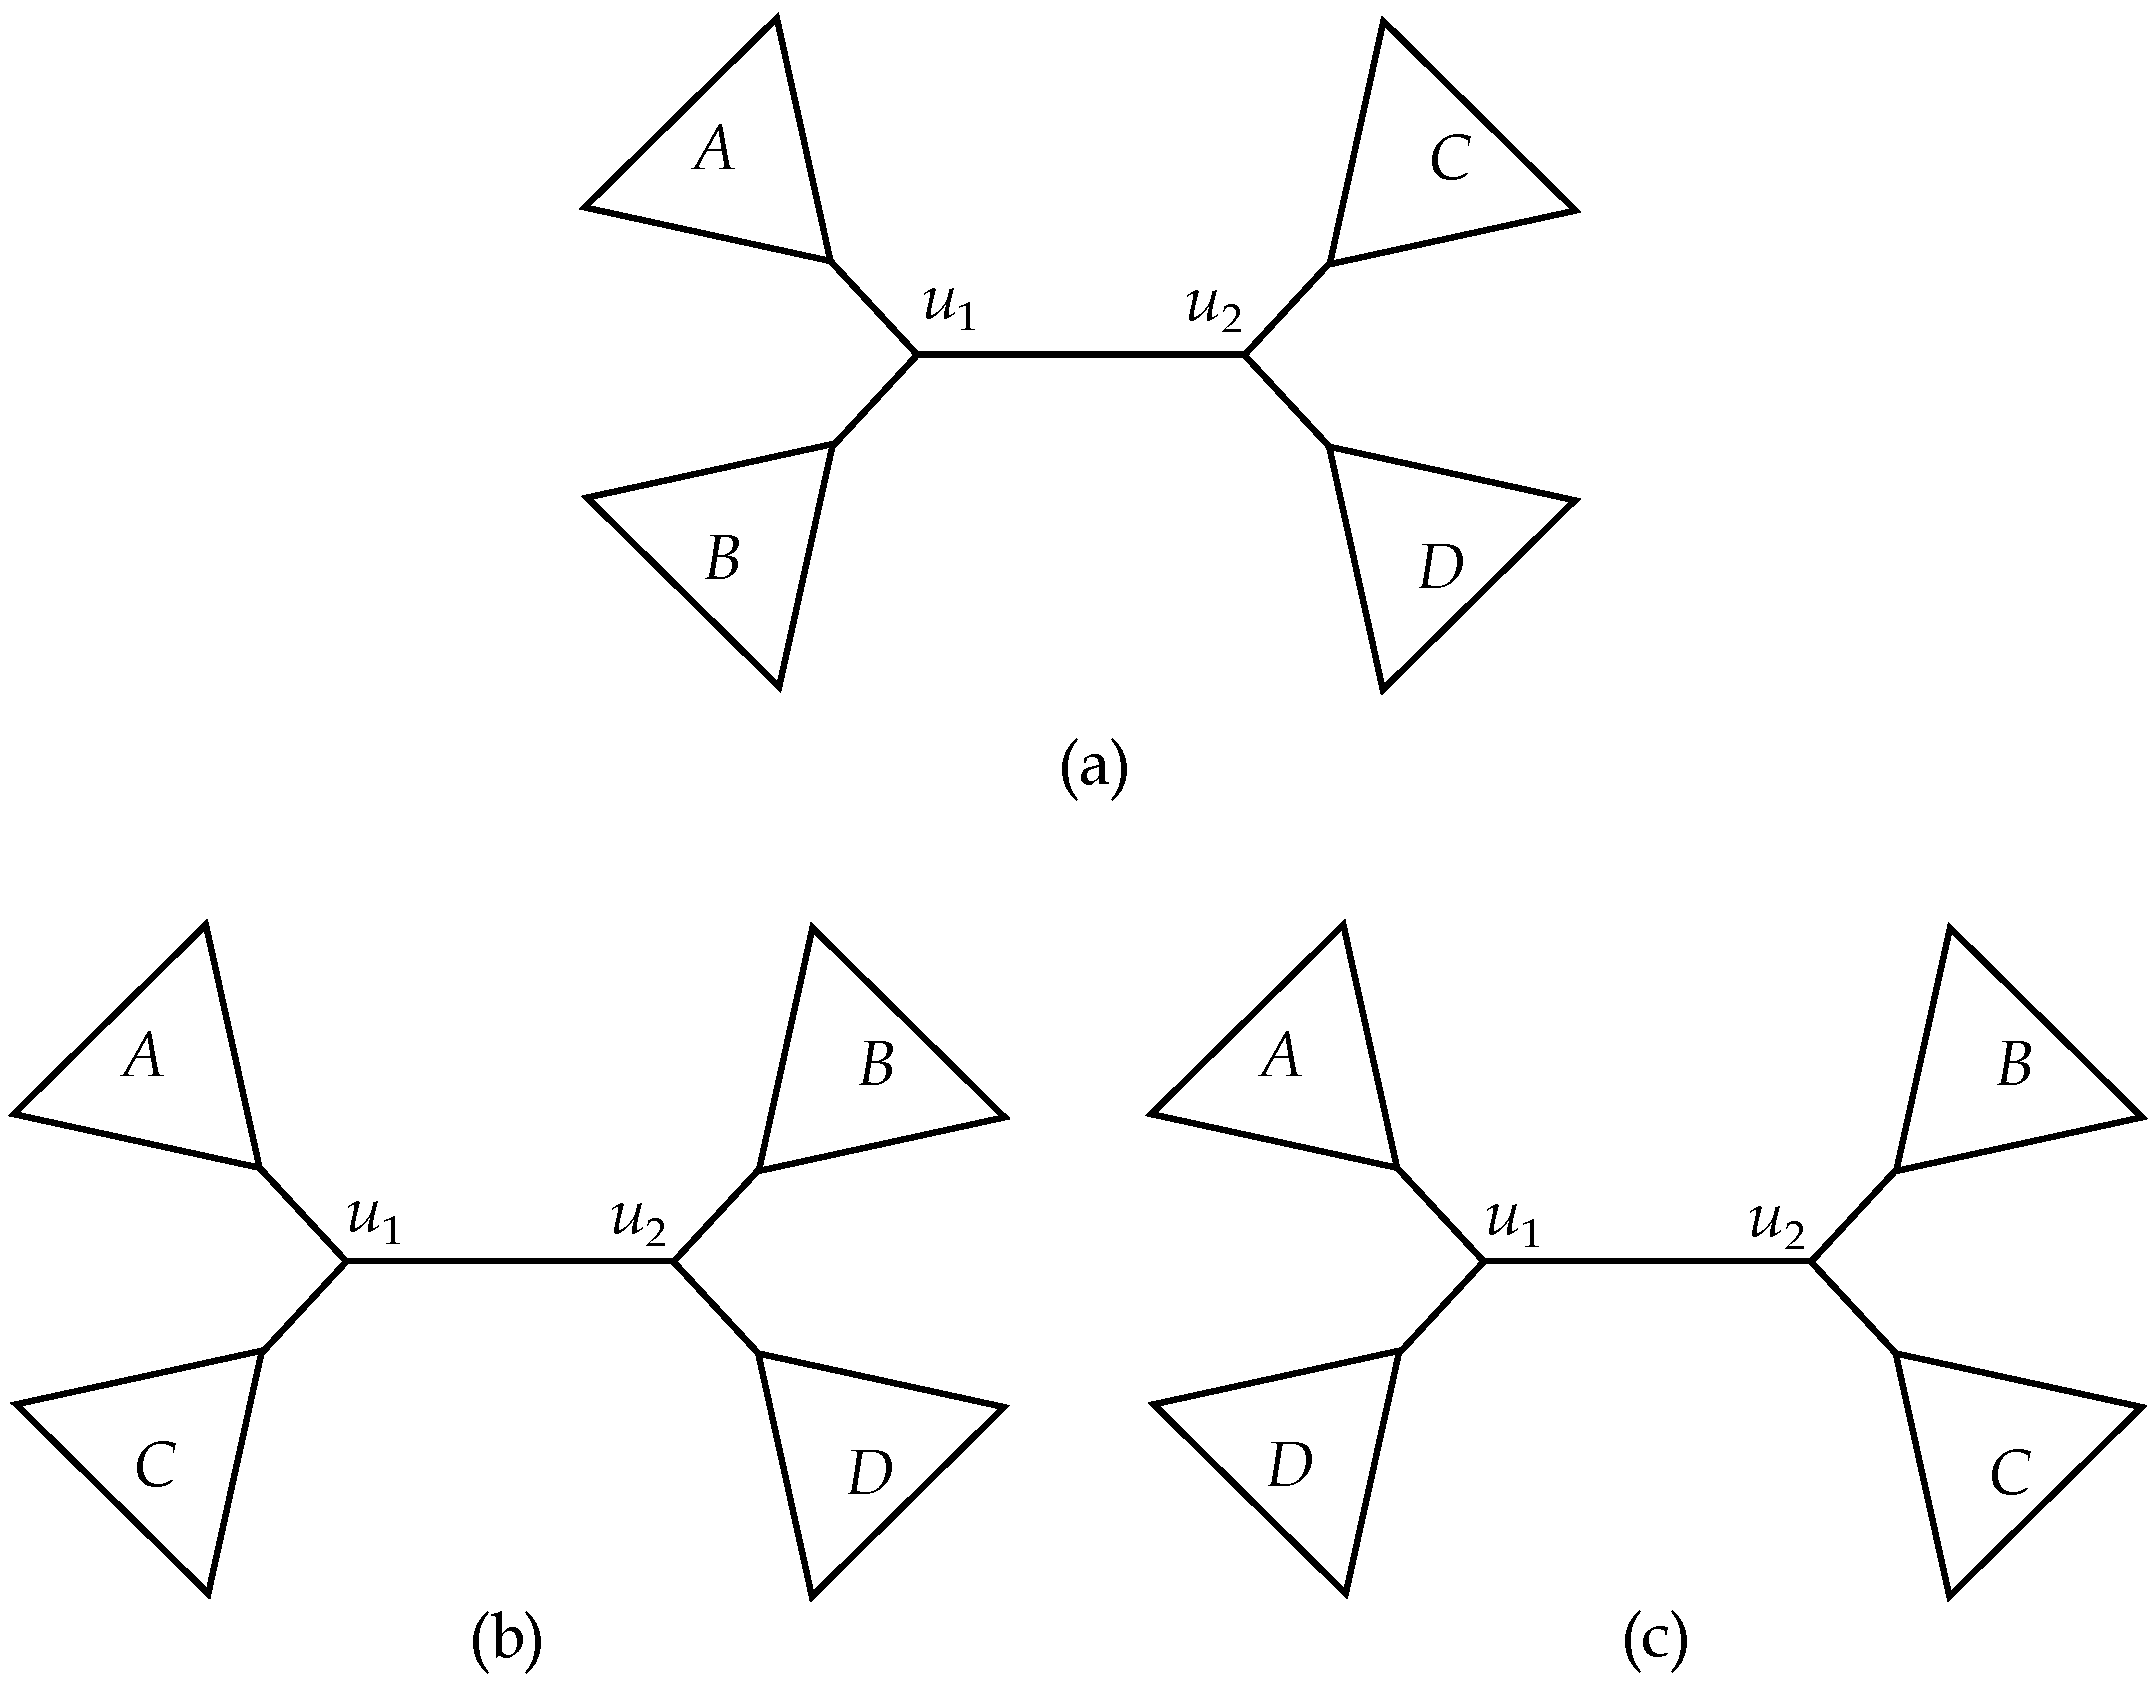
\includegraphics[scale=0.3]{Figure3.pdf}
		\caption{\textbf{Nearest Neighbor Interchange (NNI) move on an internal edge.} (a)
			A species tree ST, and (b)-(c) the neighbors of ST resulting from one NNI move on edge
			e = (u1, u2). A, B, C, and D are the sets of taxa in the four subtrees around edge e.}
	\end{figure}
	
	\subsection{Figures}
	We intend to put Figure 1 at the top of a page.
	
	\subsection{Equations}
	
\begin{equation}
	\begin{split}
		\mathcal{NQ}(n1,n2,n3) & = \binom{n_1}{2}\binom{n_2}{1}\binom{n_3}{1}+ \binom{n_2}{2}\binom{n_1}{1}\binom{n_3}{1} + \binom{n_3}{2}\binom{n_1}{1}\binom{n_2}{1} \\
		& = \frac{n_1n_2n_3(n1 + n2 + n3 + 3)}{2}
	\end{split}
\end{equation}
	
	\section{Conclusion}
	The major objectives of this assignment are listed below (please do not ignore the font sizes).

	%Unordered list
	%Ordered list -> \begin{enumerate}
	
	\begin{itemize}
		{ \Large \item To assess the ability of the students in preparing manuscripts in \LaTeX.}
		{  \item To see if the students have adequately practiced different aspects of
			writing in \LaTeX.}
		{\item To see if the students can add various basic components (e.g., tables, figures, equations) to a \LaTeX manuscript.}	
		\newpage		
		{\small \item To see if the students can leverage the available materials (both offline and online) to do
		something which has not explicitly been taught in the class.}		
	\end{itemize}	

\end{document}
